\documentclass[12pt]{article}
\usepackage{amsmath}
\usepackage{amsthm}
\usepackage{algorithm}
\usepackage{algpseudocode}
\usepackage{amssymb}
\usepackage{graphicx}
\graphicspath{ {assets/} }

\begin{document}

\title{Assignment 2 - Triangulation and Linear Programming}
\author{
	Pattarawat Chormai - 0978675 \\
}
\maketitle

\section*{Q2}

A polygon $P=(V,E)$, which has $n$ vertices and edges, can be covered by a guard if and only if there is a feasible region $R$ in
which when we place a guard, he can see every edges of the polygon. Such a region
can simply computed by using half plane intersected technic which we use for solving linear programming. \\

We first compute a half plane $h(e_i)$ of each edge $e_i$ of $P$ where a half plane corresponds to
region of the polygon. Also, the leftmost, topmost, rightmost and bottommost vertices of $P$ are used to define the
boundary box. In each step of adding $h(e_i)$, the algorithm determines whether
the current intersected region $R_{i-1}$ corresponding to $h(e_{i})$ by checking whether a helper point $v_{i-1}$
is in $h(e_i)$ or not. If not, a line $L$ moving along $x$-axis is used as a objective function of $1dBoundedLP$,
the algorithm from 4th lecture, for checking the possibility of having a new intersected region
and update $v_i$ if it is able to do so. On the other hand, if $v_{i-i}$ is in $h(e_i)$, the algorithm will do nothing because
the current intersected region is still valid. Hence, it set $v_i$ equal to $v_{i-1}$.

If the algorithm succeeds to find $v_i$ until the end, then only one guard is needed
to cover $P$, otherwise, we need more than one guard to cover $P$.


The algorithm works as follow :

\begin{center}
    \label{figure1}
    \begin{figure}[h]
    \centering
    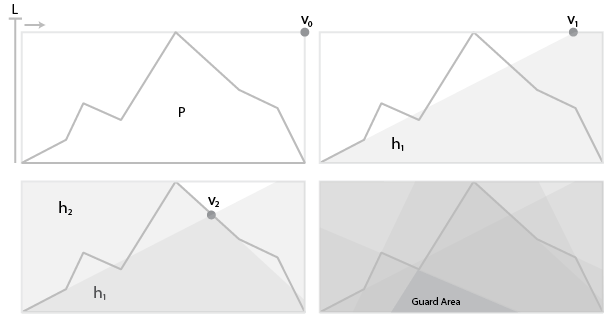
\includegraphics[width=10cm]{pat-q2}\\
    \caption{An example of how the algorithm works.} \label{fig:extremecase}
    \end{figure}
\end{center}

\begin{algorithm}[h]
  \caption{CheckOneGuardPolygon}
  \label{alg:OneGuardPolygon}
  \begin{algorithmic}
    \Require a simple polygon $P=(V,E)$
    \State Find the boundary box $R_o$ of $P$.
    \State Find $v_o$ from $R_o$
    \State Derive $h(e_i)$ for all $e_i \in E$.
    \State Shuffle $h(e_i)$ randomly for all $e_i \in E$.
    \For{$ 1 \le i \le n$}
        \If{$v_{i-1} \in h(e_i)$}
        \State $v_i \leftarrow v_{i-1}$
        \Else
            \State $\sigma $ $\leftarrow$  all intersected points of $R_{i-1}$.
            \State $v_i$ $\leftarrow$ 1dBoundedLP( $\sigma$, line equation of $h(e_i)$ )
            \If{$v_i$ = nill}
                \State return false
            \EndIf
        \EndIf
    \EndFor
    \State return true
  \end{algorithmic}
\end{algorithm}

\subsection*{Correctness}
We first argue that for any $e_i$, a guard can see it if he is in the region of $h(e_i)$.
This implies that if $P$ has a intersected region between all $h(e_i)$, then one guard is
sufficient to cover $P$. \\

The algorithm uses $v_i$ as a helper point to represent the current intersected region, whenever
the intersected region changes, $v_i$  is updated. \\

First considering $e_1$, it can be covered by a guard, if the guard is in any area of $h(e_1)$, of course this
area should be inside $P$. Assume when processing $e_i$, the intersected region between
$h(E_{i-1})$ where $E_{i-1}$ is $\{ e_j : e_j \in E \text{ and }1 \le j \le i -1 \} $ has computed already.
Thus if we put a guard in any position in the region $R_{i-1}$, he can cover all edges in $E_{i-1}$. If
the intersection of $h(e_i)$ and $h(E_{i-1})$ does not change, $v_{i-1}$ in $h(e_i)$,
one guard is still sufficient to cover $E_i$. On the other hand, if $h(e_i)$ and $h(E_{i-1})$ create
a new intersected region, $v_{i-1} \notin h(e_i)$, the algorithm will try to find a new position
for $v_i$ which represents the new intersected region. If it succeeds, only one guard
is needed to cover $E_i$, otherwise it will return false which means we need more
than one guard to cover the region. The reasoning is also true when processing  $e_n$. \\

Therefore, by using induction, the algorithm reports correct result.

\subsection*{Running Time}
\begin{itemize}
    \item Finding the boundary box takes $O(n)$.
    \item Finding $v_0$  takes constant time.
    \item Deriving half planes for all edge takes $O(n)$.
    \item Shuffling half planes order takes $O(n)$.
    \item Processing $h(e_i)$ takes \\
    $\;\;$ $O(1)$ if the intersected region does not change when processing $h(e_i)$\\
    $\;\;$ $O(i)$ otherwise, because we have to find the new position of the helper point $v_i$
\end{itemize}
Since we know that, the probability of $v_{i-1}$ and $v_i$, $Pr[v_{i-1} \in R_i]$, are the same is never greater than 1
, while the probability that we have to find new position of $v_i$, $Pr[v_{i-1} \notin R_i]$, is equal to the probability
of removing $h(e_i)$ and $v_i$ is changed, the probability of such a case is never
greater than the probability of selecting 2 half planes defining their intersected.

Thus, the expected running time is :

\begin{align*}
    T(n) &= 3O(n) + \sum_{i=1}^{n}( Pr[v_{i-1} \in R_i]*O(1) + Pr[v_{i-1} \notin R_i]*O(i) ) \\
         &= 3O(n) + O(n) + \sum_{i=1}^{n}(2/i)O(i) \\
         &= 4O(n) + 2O(n) \\
         &= O(n)
\end{align*}

Therefore, the algorithm runs in linear expected running time.

\end{document}
